\section{mo\-Rand\-Impr\-Select$<$ M $>$ Class Template Reference}
\label{classmo_rand_impr_select}\index{moRandImprSelect@{moRandImprSelect}}
One of the possible {\bf mo\-Move}{\rm (p.\,\pageref{classmo_move})} selector ({\bf mo\-Move\-Select}{\rm (p.\,\pageref{classmo_move_select})}).  


{\tt \#include $<$mo\-Rand\-Impr\-Select.h$>$}

Inheritance diagram for mo\-Rand\-Impr\-Select$<$ M $>$::\begin{figure}[H]
\begin{center}
\leavevmode
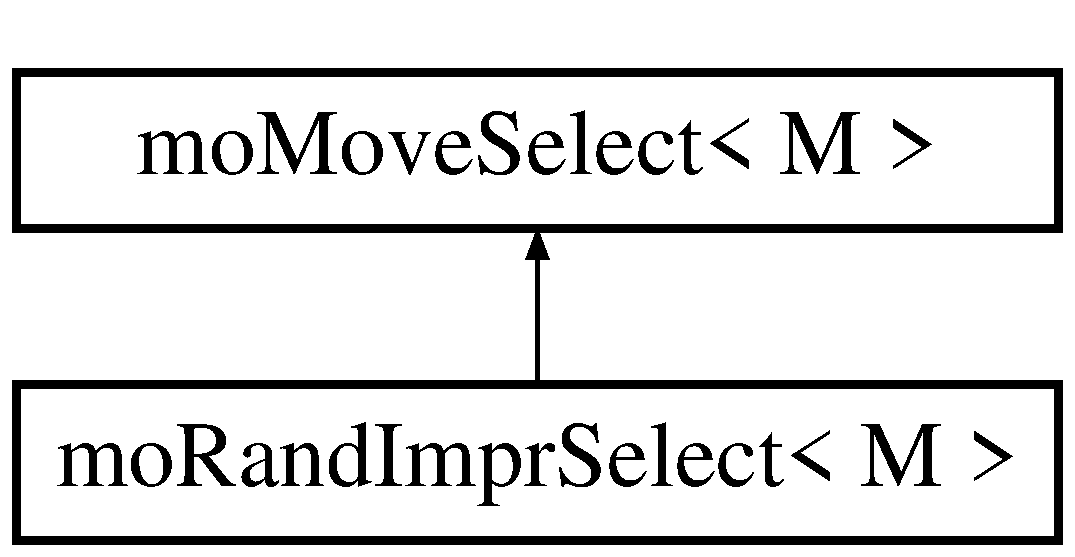
\includegraphics[height=2cm]{classmo_rand_impr_select}
\end{center}
\end{figure}
\subsection*{Public Types}
\begin{CompactItemize}
\item 
typedef M::EOType::Fitness {\bf Fitness}\label{classmo_rand_impr_select_3bff2fdb963297430543c82ffb567a5c}

\begin{CompactList}\small\item\em Alias for the fitness. \item\end{CompactList}\end{CompactItemize}
\subsection*{Public Member Functions}
\begin{CompactItemize}
\item 
void {\bf init} (const {\bf Fitness} \&\_\-\_\-fit)
\begin{CompactList}\small\item\em Procedure which all that needs a {\bf mo\-Rand\-Impr\-Select}{\rm (p.\,\pageref{classmo_rand_impr_select})}. \item\end{CompactList}\item 
bool {\bf update} (const M \&\_\-\_\-move, const {\bf Fitness} \&\_\-\_\-fit)
\begin{CompactList}\small\item\em Function that updates the fitness and move vectors. \item\end{CompactList}\item 
void {\bf operator()} (M \&\_\-\_\-move, {\bf Fitness} \&\_\-\_\-fit)  throw (Empty\-Selection)
\begin{CompactList}\small\item\em The move selection. \item\end{CompactList}\end{CompactItemize}
\subsection*{Private Attributes}
\begin{CompactItemize}
\item 
{\bf Fitness} {\bf init\_\-fit}\label{classmo_rand_impr_select_d153c277a0a2ea95ac484210d445b40e}

\begin{CompactList}\small\item\em Fitness of the current solution. \item\end{CompactList}\item 
std::vector$<$ {\bf Fitness} $>$ {\bf vect\_\-better\_\-fit}\label{classmo_rand_impr_select_05c7c3b858e8a25632f2f5c86b0c97a3}

\begin{CompactList}\small\item\em Candidate fitnesse vector. \item\end{CompactList}\item 
std::vector$<$ M $>$ {\bf vect\_\-better\_\-moves}\label{classmo_rand_impr_select_2ace12bd179144fa71d56324694201f5}

\begin{CompactList}\small\item\em Candidate move vector. \item\end{CompactList}\end{CompactItemize}


\subsection{Detailed Description}
\subsubsection*{template$<$class M$>$ class mo\-Rand\-Impr\-Select$<$ M $>$}

One of the possible {\bf mo\-Move}{\rm (p.\,\pageref{classmo_move})} selector ({\bf mo\-Move\-Select}{\rm (p.\,\pageref{classmo_move_select})}). 

All the neighbors are considered. One of them that enables an improvment of the objective function is choosen. 



Definition at line 25 of file mo\-Rand\-Impr\-Select.h.

\subsection{Member Function Documentation}
\index{moRandImprSelect@{mo\-Rand\-Impr\-Select}!init@{init}}
\index{init@{init}!moRandImprSelect@{mo\-Rand\-Impr\-Select}}
\subsubsection{\setlength{\rightskip}{0pt plus 5cm}template$<$class M$>$ void {\bf mo\-Rand\-Impr\-Select}$<$ M $>$::init (const {\bf Fitness} \& {\em \_\-\_\-fit})\hspace{0.3cm}{\tt  [inline, virtual]}}\label{classmo_rand_impr_select_a19726a1509cff874801615d63a3b5d9}


Procedure which all that needs a {\bf mo\-Rand\-Impr\-Select}{\rm (p.\,\pageref{classmo_rand_impr_select})}. 

Give a value to the initialise fitness. Clean the move and fitness vectors.

\begin{Desc}
\item[Parameters:]
\begin{description}
\item[{\em \_\-\_\-fit}]the current best fitness \end{description}
\end{Desc}


Implements {\bf mo\-Move\-Select$<$ M $>$} {\rm (p.\,\pageref{classmo_move_select_bca4c43f13d26eca7163aeb272a4a52e})}.

Definition at line 40 of file mo\-Rand\-Impr\-Select.h.

References mo\-Rand\-Impr\-Select$<$ M $>$::init\_\-fit, mo\-Rand\-Impr\-Select$<$ M $>$::vect\_\-better\_\-fit, and mo\-Rand\-Impr\-Select$<$ M $>$::vect\_\-better\_\-moves.\index{moRandImprSelect@{mo\-Rand\-Impr\-Select}!update@{update}}
\index{update@{update}!moRandImprSelect@{mo\-Rand\-Impr\-Select}}
\subsubsection{\setlength{\rightskip}{0pt plus 5cm}template$<$class M$>$ bool {\bf mo\-Rand\-Impr\-Select}$<$ M $>$::update (const M \& {\em \_\-\_\-move}, const {\bf Fitness} \& {\em \_\-\_\-fit})\hspace{0.3cm}{\tt  [inline, virtual]}}\label{classmo_rand_impr_select_60ae5548560caee7e28d5ed2446186c9}


Function that updates the fitness and move vectors. 

if a move give a better fitness than the initial fitness, it is saved and the fitness too.

\begin{Desc}
\item[Parameters:]
\begin{description}
\item[{\em \_\-\_\-move}]a new move. \item[{\em \_\-\_\-fit}]a new fitness associated to the new move. \end{description}
\end{Desc}
\begin{Desc}
\item[Returns:]TRUE. \end{Desc}


Implements {\bf mo\-Move\-Select$<$ M $>$} {\rm (p.\,\pageref{classmo_move_select_7c157b6e64fd417acf6e900059204eb1})}.

Definition at line 56 of file mo\-Rand\-Impr\-Select.h.

References mo\-Rand\-Impr\-Select$<$ M $>$::init\_\-fit, mo\-Rand\-Impr\-Select$<$ M $>$::vect\_\-better\_\-fit, and mo\-Rand\-Impr\-Select$<$ M $>$::vect\_\-better\_\-moves.\index{moRandImprSelect@{mo\-Rand\-Impr\-Select}!operator()@{operator()}}
\index{operator()@{operator()}!moRandImprSelect@{mo\-Rand\-Impr\-Select}}
\subsubsection{\setlength{\rightskip}{0pt plus 5cm}template$<$class M$>$ void {\bf mo\-Rand\-Impr\-Select}$<$ M $>$::operator() (M \& {\em \_\-\_\-move}, {\bf Fitness} \& {\em \_\-\_\-fit})  throw ({\bf Empty\-Selection})\hspace{0.3cm}{\tt  [inline]}}\label{classmo_rand_impr_select_5ee57f77a450c0a9ce50bfccf3ad2a55}


The move selection. 

One the saved move is randomly chosen.

\begin{Desc}
\item[Parameters:]
\begin{description}
\item[{\em \_\-\_\-move}]the reference of the move that can be initialised by the function. \item[{\em \_\-\_\-fit}]the reference of the fitness that can be initialised by the function. \end{description}
\end{Desc}
\begin{Desc}
\item[Exceptions:]
\begin{description}
\item[{\em {\bf Empty\-Selection}{\rm (p.\,\pageref{class_empty_selection})}}]If no move which improves the current fitness are found. \end{description}
\end{Desc}


Definition at line 77 of file mo\-Rand\-Impr\-Select.h.

References mo\-Rand\-Impr\-Select$<$ M $>$::vect\_\-better\_\-fit, and mo\-Rand\-Impr\-Select$<$ M $>$::vect\_\-better\_\-moves.

The documentation for this class was generated from the following file:\begin{CompactItemize}
\item 
mo\-Rand\-Impr\-Select.h\end{CompactItemize}
